\section[Buffer Manager Page Eviction]{Page Eviction by the Buffer Pool Management}

\frame{\sectionpage}

\subsection{Introduction}

\begin{frame}
    \frametitle{The Buffer Pool}

    \newcommand{\bufferPage}[3]{%
        \node[db page, ####3] (####1) {\ensuremath{P_{####2}^{\prime}}};
    }
    \newcommand{\hddPage}[3]{%
        \node[db page, ####3] (####1) {\ensuremath{P_{####2}}};
    }
    \tikzset{%
        db page/.style = {draw = structure,
                          fill = structure!15,
                          rectangle,
                          rounded corners = 1pt,
                          thick,
                          minimum width = 2.5em,
                          minimum height = 5ex},
        node distance = 2ex
    }

    \centering
    \begin{tikzpicture}
        \bufferPage{b5}{5}{at = {(0, 0)}}
        \bufferPage{b2}{2}{below = of b5}
        \bufferPage{b1}{1}{right = of b5}
        \bufferPage{b8}{8}{right = of b2}
        \begin{scope}[on background layer]
            \node[draw = black, rectangle, rounded corners = 2.5pt, very thick, fill = black!15, fit = (b5) (b8), label = {\textcolor{structure}{Buffer pool}}] (buffer) {};
        \end{scope}

        \hddPage{s4}{4}{right = 15ex of buffer}
        \hddPage{s1}{1}{above = of s4}
        \hddPage{s7}{7}{below = of s4}
        \hddPage{s2}{2}{right = of s1}
        \hddPage{s3}{3}{right = of s2}
        \hddPage{s5}{5}{right = of s4}
        \hddPage{s6}{6}{right = of s5}
        \hddPage{s8}{8}{right = of s7}
        \hddPage{s9}{9}{right = of s8}
        \begin{scope}[on background layer]
            \node[draw = black, cylinder, shape border rotate = 90, shape aspect = .375, very thick, left color = black!25, right color = black!25, middle color = black!15, fit = (s1) (s9), label = {\textcolor{structure}{SSD}}] (ssd) {};
        \end{scope}

        \node[cloud, thick, draw = black!50, above = 7.5ex of buffer, minimum width = 7.5em, minimum height = 10ex] (layers) {\Large...};

        \draw[-latex, very thick] (buffer) edge[bend right = 20] node[below] {evict} (ssd);
        \draw[-latex, very thick] (ssd) edge[bend right = 20] node[above] {fetch} (buffer);
        \draw[-latex, very thick] (layers) edge[bend right = 40] node[left] {fix} (buffer);
        \draw[-latex, very thick] (layers) edge[bend left = 40] node[right] {unfix} (buffer);
    \end{tikzpicture}
\end{frame}

\begin{frame}
    \frametitle[Extended Classification by Effelsberg and Härder]{Extended Page Replacement Algorithm Classification by Effelsberg and Härder From \cite{Effelsberg:1984}}

    \renewcommand{\baselinestretch}{.6}
    \setcellgapes{2pt}
    \setlength\arrayrulewidth{.6pt}
    \color{section in head/foot.bg}
    \makegapedcells
    \footnotesize
    \resizebox{\textwidth}{!}{
        \begin{tabular}{|c|c|c|c|c|c|}
            \hline
            \multicolumn{2}{|c|}{%
                \multirow{2}{*}{%
                    \textcolor{structure}{%
                        \textbf{%
                            \makecell[c]{%
                                Consideration\\%
                                during selection\\%
                                decision%
                            }%
                        }%
                    }%
                }%
            }                                   &
            \multicolumn{4}{c|}{%
                \textcolor{structure}{%
                    \textbf{Age}%
                }%
            }                                                       \\ \cline{3-6}
            \multicolumn{2}{|c|}{}              &
            \textcolor{structure}{%
                \makecell[c]{%
                    No\\%
                    consideration%
                }%
            }                                   &
            \textcolor{structure}{%
                \makecell[c]{%
                    Since most\\%
                    recent reference%
                }%
            }                                   &
            \uncover<2->{%
                \textcolor{structure}{%
                    \makecell[c]{%
                        Since some\\%
                        recent reference%
                    }%
                }%
            }                                   &
            \textcolor{structure}{%
                \makecell[c]{%
                    Since first\\%
                    reference%
                }%
            }                                                       \\ \hline
            \multirow{4}{*}{%
                \rotcell[c]{%
                    \textcolor{structure}{%
                        \textbf{References}%
                    }%
                }%
            }                                   &
            \textcolor{structure}{%
                \makecell[c]{%
                    No\\%
                    consideration%
                }%
            }                                   &
            \uncover<4->{%
                \textcolor{normal text.fg}{%
                    RANDOM%
                }%
            }                                   &
                                                &
                                                &
            \textcolor{normal text.fg}{%
                \makecell[c]{%
                    \uncover<5->{FIFO}\\%
                    \uncover<6->{FILO}%
                }%
            }                                                       \\ \cline{2-6}
                                                &
            \textcolor{structure}{%
                \makecell[c]{%
                    Most recent\\%
                    reference%
                }%
            }                                   &
            \textcolor{normal text.fg}{%
                \uncover<12->{ZCLOCK}%
            }                                   &
            \textcolor{normal text.fg}{%
                \makecell[c]{%
                    \uncover<7->{LRU}\\%
                    \uncover<8->{MRU}\\%
                    \uncover<11->{CLOCK}\\%
                    \uncover<14->{GCLOCK-V2}\\%
                    \uncover<16->{DGCLOCK-V2}\\%
                    \uncover<21->{LeanStore}%
                }%
            }                                   &
                                                &
                                                                    \\ \cline{2-6}
                                                &
            \uncover<3->{%
                \textcolor{structure}{%
                    \makecell[c]{%
                        Some recent\\%
                        references%
                    }%
                }%
            }                                   &
                                                &
            \textcolor{normal text.fg}{%
                \uncover<10->{SLRU}%
            }                                   &
            \textcolor{normal text.fg}{%
                \makecell[c]{%
                    \uncover<9->{LRU-K}\\%
                    \uncover<20->{LRD-V2}%
                }%
            }                                   &
                                                                    \\ \cline{2-6}
                                                &
            \textcolor{structure}{%
                \makecell[c]{%
                    All\\%
                    references%
                }%
            }                                   &
            \textcolor{normal text.fg}{%
                \uncover<17->{LFU}%
            }                                   &
            \textcolor{normal text.fg}{%
                \makecell[c]{%
                    \uncover<13->{GCLOCK-V1}\\%
                    \uncover<15->{DGCLOCK-V1}%
                }%
            }                                   &
                                                &
            \textcolor{normal text.fg}{%
                    \makecell[c]{%
                    \uncover<19->{LRD-V1}\\%
                    \uncover<18->{LFUDA}%
                }%
            }                                                       \\ \hline
        \end{tabular}
    }
\end{frame}

\subsection[LRU]{Least Recently Used}

\frame{\subsectionpage}

\subsubsection[Hash-Map-Doubly-Linked-List]{Hash-Map-Doubly-Linked-List Implementation}

\frame{\subsubsectionpage}

\begin{frame}
    \frametitle{Hash-Map-Doubly-Linked-List}

    \tikzset{%
        queueelement/.style = {draw = black,
                               rectangle},
        queuereferences/.style = {draw = black,
                                  rectangle split,
                                  rectangle split parts = 2,
                                  rectangle split horizontal,
                                  text = black!75,
                                  inner xsep = .75pt}
    }
    \newcommand{\queueelement}[4]{%
        \node [{queuereferences, ####4}] ({####2})%
            {####1\nodepart{two}####3};%
        \node [queueelement, above = -.6pt of {####2}] (center####2) {\textbf{####2}};
    }
    \newcommand{\getAngle}[2]{%
        \pgfmathanglebetweenpoints{\pgfpointanchor{####1}{center}}{\pgfpointanchor{####2}{center}}
        \global\let\calculatedAngle\pgfmathresult
    }

    \Wider{%
        \centering
        \resizebox{\linewidth}{!}{%
            \begin{tikzpicture}[>=latex,
                                semithick,
                                node distance = 1em]
                % Draw the hash map root:
                \node [draw = black, rectangle, thick] (hashmap) {hashMap};

                % Draw the queue elements:
                \node [below = 10em of hashmap] (center) {};
                \queueelement{7}{0}{6}{left = .5em of center.base}
                \queueelement{10}{7}{0}{left = of 0}
                \queueelement{2}{10}{7}{left = of 7}
                \queueelement{14}{2}{10}{left = of 10}
                \queueelement{15}{14}{2}{left = of 2}
                \queueelement{9}{15}{14}{left = of 14}
                \queueelement{8}{9}{15}{left = of 15}
                \queueelement{NULL}{8}{9}{left = of 9}
                \queueelement{0}{6}{13}{right = .5em of center.base}
                \queueelement{6}{13}{1}{right = of 6}
                \queueelement{13}{1}{5}{right = of 13}
                \queueelement{1}{5}{3}{right = of 1}
                \queueelement{5}{3}{12}{right = of 5}
                \queueelement{3}{12}{11}{right = of 3}
                \queueelement{12}{11}{4}{right = of 12}
                \queueelement{11}{4}{NULL}{right = of 11}



                % Draw the arrows to the queue elements:
                \foreach \element in {0, 1, ..., 15} {%
                    \getAngle{hashmap}{center\element}
                    \draw [->] (hashmap) to [in = 90, out = \calculatedAngle, looseness = .75] (center\element.north);
                }

                % Draw the arrows between the queue elements:
                \draw [->, draw = black!50]  (8) to [in = 180, out = 0]  (center9);
                \draw [->, draw = black!50]  (9) to [in = 180, out = 0] (center15);
                \draw [->, draw = black!50] (15) to [in = 180, out = 0] (center14);
                \draw [->, draw = black!50] (14) to [in = 180, out = 0]  (center2);
                \draw [->, draw = black!50]  (2) to [in = 180, out = 0] (center10);
                \draw [->, draw = black!50] (10) to [in = 180, out = 0]  (center7);
                \draw [->, draw = black!50]  (7) to [in = 180, out = 0]  (center0);
                \draw [->, draw = black!50]  (0) to [in = 180, out = 0]  (center6);
                \draw [->, draw = black!50]  (6) to [in = 180, out = 0] (center13);
                \draw [->, draw = black!50] (13) to [in = 180, out = 0]  (center1);
                \draw [->, draw = black!50]  (1) to [in = 180, out = 0]  (center5);
                \draw [->, draw = black!50]  (5) to [in = 180, out = 0]  (center3);
                \draw [->, draw = black!50]  (3) to [in = 180, out = 0] (center12);
                \draw [->, draw = black!50] (12) to [in = 180, out = 0] (center11);
                \draw [->, draw = black!50] (11) to [in = 180, out = 0, in looseness = 2]  (center4);
                \draw [->, draw = black!50]  (4) to [in = 0, out = 180] (center11);
                \draw [->, draw = black!50] (11) to [in = 0, out = 180] (center12);
                \draw [->, draw = black!50] (12) to [in = 0, out = 180]  (center3);
                \draw [->, draw = black!50]  (3) to [in = 0, out = 180]  (center5);
                \draw [->, draw = black!50]  (5) to [in = 0, out = 180]  (center1);
                \draw [->, draw = black!50]  (1) to [in = 0, out = 180] (center13);
                \draw [->, draw = black!50] (13) to [in = 0, out = 180]  (center6);
                \draw [->, draw = black!50]  (6) to [in = 0, out = 180]  (center0);
                \draw [->, draw = black!50]  (0) to [in = 0, out = 180]  (center7);
                \draw [->, draw = black!50]  (7) to [in = 0, out = 180] (center10);
                \draw [->, draw = black!50] (10) to [in = 0, out = 180]  (center2);
                \draw [->, draw = black!50]  (2) to [in = 0, out = 180] (center14);
                \draw [->, draw = black!50] (14) to [in = 0, out = 180] (center15);
                \draw [->, draw = black!50] (15) to [in = 0, out = 180]  (center9);
                \draw [->, draw = black!50]  (9) to [in = 0, out = 180, in looseness = 2]  (center8);

                \node (head)     [draw = black, rectangle, text = black!75, above = 4em of center8] {8};
                \node (headname) [above = .125em of head]                                           {head};
                \draw [->, draw = black!50] (head) to [bend right]  (center8);
                \node (tail)     [draw = black, rectangle, text = black!75, above = 4em of center4] {4};
                \node (tailname) [above = .125em of tail]                                           {tail};
                \draw [->, draw = black!50] (tail) to [bend  left]  (center4);
            \end{tikzpicture}%
        }%
    }
\end{frame}

\subsubsection[Timestamp-Sorting]{Timestamp-Sorting Implementation}

\frame{\subsubsectionpage}

\begin{frame}
    \frametitle{Page Reference Statistics}

    \tikzset{%
        timestampfield/.style = {draw = black,
            rectangle,
            fill = black!10},
        sortfield/.style = {draw = black,
            rectangle split,
            rectangle split horizontal,
            rectangle split parts = 2,
            fill = black!10}
    }

    \centering
    \resizebox{\linewidth}{!}{%
        \begin{tikzpicture}[>=latex,
            semithick,
            node distance = 1em]
            \node[timestampfield, label = left:0] (liveTimestamp0) {\textls[-50]{2020-09-14 12:34:56.197548}};
            \foreach \timestampnumber/\previoustimestampnumber/\timestamp in {1/0/2020-09-14 12:34:56 821122,
                2/1/2020-09-14 12:34:57 062836,
                3/2/2020-09-14 12:34:56 227794,
                4/3/2020-09-14 12:34:57 289365,
                5/4/2020-09-14 12:34:56 849729,
                6/5/2020-09-14 12:34:56 377511,
                7/6/2020-09-14 12:34:57 179364,
                8/7/2020-09-14 12:34:56 498737,
                9/8/2020-09-14 12:34:56 776239,
                10/9/2020-09-14 12:34:56 720335,
                11/10/2020-09-14 12:34:56 855806,
                12/11/2020-09-14 12:34:56 213471,
                13/12/2020-09-14 12:34:56 881209,
                14/13/2020-09-14 12:34:56 346659,
                15/14/2020-09-14 12:34:56 793698}
            \node[timestampfield, below = -.8pt of liveTimestamp\previoustimestampnumber, label = left:\timestampnumber] (liveTimestamp\timestampnumber) {\textls[-50]{\timestamp}};
            \node[draw = none, above = 0em of liveTimestamp0] (liveTimestampName) {liveTimestamps};
            
            \node[sortfield, right = 1.5em of liveTimestamp0] (sort00) {\phantom{0}2\nodepart{two}\textls[-50]{2020-09-14 12:34:56 071309}};
            \foreach \timestampnumber/\frameindex/\timestamp in {1/\phantom{0}0/2020-09-14 12:34:56.197548,
                2/12/2020-09-14 12:34:56 213471,
                3/\phantom{0}3/2020-09-14 12:34:56 227794,
                4/14/2020-09-14 12:34:56 346659,
                5/\phantom{0}6/2020-09-14 12:34:56 377511,
                6/\phantom{0}8/2020-09-14 12:34:56 498737,
                7/10/2020-09-14 12:34:56 720335,
                8/\phantom{0}9/2020-09-14 12:34:56 776239,
                9/15/2020-09-14 12:34:56 793698,
                10/\phantom{0}1/2020-09-14 12:34:56 821122,
                11/\phantom{0}5/2020-09-14 12:34:56 849729,
                12/11/2020-09-14 12:34:56 855806,
                13/\phantom{0}4/2020-09-14 12:34:56 865145,
                14/13/2020-09-14 12:34:56 881209,
                15/\phantom{0}7/2020-09-14 12:34:56 987742}
            \node[sortfield, right = 1.5em of liveTimestamp\timestampnumber] (sort0\timestampnumber) {\frameindex\nodepart{two}\textls[-50]{\timestamp}};
            \node[draw = none, above = 0em of sort00] (sort0Name) {LRUqueue0};
            \node[draw = none, below = .25em of sort015] {%
                \begin{tikzpicture}
                    \node[draw = black, rectangle, fill = black!10] (useSort0) {true};
                    \node[draw = none, left = .3333em of useSort0.base west, anchor = base east] (useSort0Name) {useLRUqueue0};
                \end{tikzpicture}
            };
            
            \node[sortfield, right = 1.5em of sort00] (sort10) {\phantom{1}8\nodepart{two}\textls[-50]{2020-09-14 12:34:55 185406}};
            \foreach \timestampnumber/\frameindex/\timestamp in {1/\phantom{0}9/2020-09-14 12:34:55.218616,
                2/\phantom{0}1/2020-09-14 12:34:55 222490,
                3/13/2020-09-14 12:34:55 439575,
                4/11/2020-09-14 12:34:55 582807,
                5/12/2020-09-14 12:34:55 607186,
                6/\phantom{0}5/2020-09-14 12:34:55 611986,
                7/\phantom{0}4/2020-09-14 12:34:55 688895,
                8/15/2020-09-14 12:34:55 726161,
                9/\phantom{0}7/2020-09-14 12:34:55 742479,
                10/10/2020-09-14 12:34:55 809492,
                11/\phantom{0}6/2020-09-14 12:34:55 953010,
                12/\phantom{0}3/2020-09-14 12:34:55 955357,
                13/14/2020-09-14 12:34:55 978132,
                14/\phantom{0}2/2020-09-14 12:34:56 071309,
                15/\phantom{0}0/2020-09-14 12:34:56.197548}
            \node[sortfield, right = 1.5em of sort0\timestampnumber] (sort1\timestampnumber) {\frameindex\nodepart{two}\textls[-50]{\timestamp}};
            \node[draw = none, above = 0em of sort10] (sort1Name) {LRUqueue1};
            \node[draw = none, below = .25em of sort115] {%
                \begin{tikzpicture}
                    \node[draw = black, rectangle, fill = black!10] (useSort1) {false};
                    \node[draw = none, left = .3333em of useSort1.base west, anchor = base east] (useSort1Name) {useLRUqueue1};
                \end{tikzpicture}
            };
            
            \node[draw = none, below = .5em of liveTimestamp15] (lastChecked) {%
                \begin{tikzpicture}
                    \node[draw = black, rectangle, fill = black!10] (lastChecked) {$\circ$\vphantom{f}};
                    \node[draw = none, left = .3333em of lastChecked.base west, anchor = base east] (lastCheckedName) {lastChecked};
                \end{tikzpicture}
            };
            %                \node[draw = none, below = .5em of liveTimestamp15] (lastChecked) {lastChecked};
            \draw [->, draw = black] ([xshift = -.875em, yshift = -.0625em]lastChecked.east) to ([xshift = 1em, yshift = -.0625em]lastChecked.east) to [in = 180, out = 0, in looseness = .375, out looseness = .375]  (sort00);
            
            \node[draw = none, below = 2.75em of $(liveTimestamp15)!0.5!(sort015)$] {%
                \begin{tikzpicture}
                    \node[draw = black, rectangle, fill = black!10] (sortingInProgress) {false};
                    \node[draw = none, left = .3333em of sortingInProgress.base west, anchor = base east] (sortingInProgressName) {sortingInProgress};
                \end{tikzpicture}
            };
            \node[draw = none, below = 2.75em of $(sort015)!0.5!(sort115)$] {%
                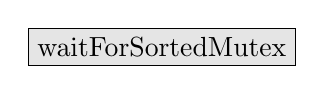
\begin{tikzpicture}
                    \node[draw = black, rectangle, fill = black!10] (waitForSortedMutexName) {waitForSortedMutex};
                \end{tikzpicture}
            };
        \end{tikzpicture}%
    }
\end{frame}

\subsection[LeanStore]{LeanStore Replacement \cite{Leis:2018}}

\frame{\subsectionpage}

\begin{frame}
    \frametitle{Basic Concept (Pointer Swizzling)}

    \tikzset{%
        state/.style = {circle, thick, draw = ####1, text = ####1, font = \bfseries}
    }

    \centering
    \begin{tikzpicture}[node distance = 12.5em]
        \node[state = black, visible on = <2->]                        (ssd)           {\makecell[c]{Cold\\(SSD)}};
        \node[state = red, below left of = ssd, visible on = <3->]     (hot)           {\makecell[c]{Hot\\(RAM)}};
        \node[state = blue, below right of = ssd, visible on = <4->]   (cold)          {\makecell[c]{Cold\\(RAM)}};

        \draw[-latex, thick, visible on = <3->]  (ssd)  edge[bend right = 10]  node[above left]  {\makecell[c]{fetch\\swizzle}} (hot);
        \draw[-latex, thick, visible on = <6->]  (cold) edge[bend right = 10]  node[above right]  {\makecell[c]{evict}}          (ssd);
        \draw[-latex, thick, visible on = <4->]  (hot)  edge[bend right = 10]  node[below] {\makecell[c]{unswizzle}}      (cold);
        \draw[-latex, thick, visible on = <5->] (cold)   edge[bend right = 10]   node[above] {\makecell[c]{swizzle}}     (hot);    
    \end{tikzpicture}\end{frame}

\begin{frame}
    \frametitle{Performance Evaluation}
    
    \pgfplotsset{%
        every axis/.append style = {
            yticklabel style = {font = \scriptsize},
            scaled y ticks = false,
            ybar = .8pt,
            bar width = .25em,
            xmin = -0.75,
            xmax = 6.75,
            xtick style = {draw = none},
            xtick = {0, 1, 2, 3, 4, 5, 6},
            xticklabels = {{\SI{0.5}{\giga\byte}}, {\SI{1}{\giga\byte}}, {\SI{2.5}{\giga\byte}}, {\SI{5}{\giga\byte}}, {\SI{10}{\giga\byte}}, {\SI{20}{\giga\byte}}, {\SI{30}{\giga\byte}}},
            x tick label style = {align = center,
                                  font = \footnotesize},
            width = .925\textwidth,
            height = .8\paperheight
        }
    }
    
    \tikzset{%
        p10/.append style = {thick, draw = Cerulean, fill = Cerulean!3},
        p25/.append style = {thick, draw = Cerulean, fill = Cerulean!7.5},
        p50/.append style = {thick, draw = Cerulean, fill = Cerulean!15},
        p75/.append style = {thick, draw = Cerulean, fill = Cerulean!22.5},
        p100/.append style = {thick, draw = Cerulean, fill = Cerulean!30},
        p150/.append style = {thick, draw = Cerulean, fill = Cerulean!45},
        p200/.append style = {thick, draw = Cerulean, fill = Cerulean!60},
        p250/.append style = {thick, draw = Cerulean, fill = Cerulean!75},
        missrate/.style = {mark = *}
    }
    
    \begin{tikzpicture}
        \begin{axis}[ymode = normal,
                     ymin = 0,
                     ymax = 1000000,
                     ymajorgrids = true,
                     yticklabel style = {/pgf/number format/fixed},
                     legend entries = {\SI{1}{\percent}, \alert<3->{\SI{2.5}{\percent}}, \SI{5}{\percent}, \SI{7.5}{\percent}, \SI{10}{\percent}, \SI{15}{\percent}, \SI{20}{\percent}, \SI{25}{\percent}},
                     legend style = {font = \tiny,
                                     legend columns = 4,
                                     /tikz/every even column/.append style = {column sep = 0.05cm},
                                     row sep = -2pt,
                                     draw = none,
                                     fill = none,
                                     at = {(0.5, 0.97)},
                                     anchor = north}]
            \addplot[p10] coordinates
                {(0, 58567.00) (1, 58268.03) (2, 66021.36) (3, 69642.80) (4, 146078.15) (5, 575054.82) (6, 887189.46)};
            \addplot[p25] coordinates
                {(0, 56933.28) (1, 61109.63) (2, 67583.42) (3, 72281.31) (4, 144405.91) (5, 574779.55) (6, 880128.90)};
            \addplot[p50] coordinates
                {(0, 57264.51) (1, 60318.40) (2, 67004.82) (3, 70148.16) (4, 146441.85) (5, 575556.58) (6, 883381.32)};
            \addplot[p75] coordinates
                {(0, 57925.46) (1, 58989.11) (2, 64552.22) (3, 69460.85) (4, 144025.08) (5, 576188.00) (6, 882856.50)};
            \addplot[p100] coordinates
                {(0, 59563.60) (1, 60740.88) (2, 65423.43) (3, 71580.94) (4, 146095.23) (5, 575680.50) (6, 883790.28)};
            \addplot[p150] coordinates
                {(0, 57593.60) (1, 59380.81) (2, 64941.56) (3, 70230.15) (4, 146845.52) (5, 575828.84) (6, 892140.47)};
            \addplot[p200] coordinates
                {(0, 59598.74) (1, 60914.58) (2, 67271.97) (3, 71998.14) (4, 145349.17) (5, 574940.67) (6, 884519.24)};
            \addplot[p250] coordinates
                {(0, 57588.15) (1, 58937.21) (2, 65513.92) (3, 68994.17) (4, 145166.72) (5, 574710.40) (6, 886323.41)};
        \end{axis}
        \begin{axis}[axis y line* = right,
                     ymode = normal,
                     ymin = 100,
                     ymax = 87.5,
                     ytick distance = 2.5,
                     grid = none,
                     ycomb = .8pt,
                     y coord trafo/.code = {
                         \pgfmathparse{100 - ####1}
                         \pgfmathresult
                     },
                     yticklabel={\SI[round-mode = places, round-precision = 0]{\tick}{\percent}}]
            \addplot[p10, missrate, xshift = 12.375*(-7/7), visible on = <2->] coordinates
                {(0, 89.25) (1, 91.76) (2, 95.48) (3, 97.81) (4, 99.53) (5, 99.84) (6, 99.86)};
            \addplot[p25, missrate, xshift = 12.375*(-5/7), visible on = <2->] coordinates
                {(0, 89.33) (1, 91.82) (2, 95.49) (3, 97.85) (4, 99.53) (5, 99.84) (6, 99.86)};
            \addplot[p50, missrate, xshift = 12.375*(-3/7), visible on = <2->] coordinates
                {(0, 89.43) (1, 91.80) (2, 95.48) (3, 97.81) (4, 99.55) (5, 99.84) (6, 99.86)};
            \addplot[p75, missrate, xshift = 12.375*(-1/7), visible on = <2->] coordinates
                {(0, 89.24) (1, 91.75) (2, 95.46) (3, 97.78) (4, 99.52) (5, 99.84) (6, 99.86)};
            \addplot[p100, missrate, xshift = 12.375*(1/7), visible on = <2->] coordinates
                {(0, 89.36) (1, 91.87) (2, 95.42) (3, 97.83) (4, 99.53) (5, 99.84) (6, 99.86)};
            \addplot[p150, missrate, xshift = 12.375*(3/7), visible on = <2->] coordinates
                {(0, 89.28) (1, 91.80) (2, 95.38) (3, 97.79) (4, 99.54) (5, 99.84) (6, 99.86)};
            \addplot[p200, missrate, xshift = 12.375*(5/7), visible on = <2->] coordinates
                {(0, 89.45) (1, 91.87) (2, 95.50) (3, 97.83) (4, 99.53) (5, 99.84) (6, 99.86)};
            \addplot[p250, missrate, xshift = 12.375*(7/7), visible on = <2->] coordinates
                {(0, 89.43) (1, 91.80) (2, 95.46) (3, 97.79) (4, 99.53) (5, 99.84) (6, 99.86)};
        \end{axis}
    \end{tikzpicture}
\end{frame}

\subsection[All]{All Page Replacement Algorithms}

\frame{\subsectionpage}

\begin{frame}
    \frametitle{Overview}
    
    \renewcommand{\baselinestretch}{.6}
    \setcellgapes{2pt}
    \setlength\arrayrulewidth{.6pt}
    \color{section in head/foot.bg}
    \makegapedcells
    \footnotesize
    \resizebox{\textwidth}{!}{
        \begin{tabular}{|c|c|c|c|c|c|}
            \hline
            \multicolumn{2}{|c|}{%
                \multirow{2}{*}{%
                    \textcolor{structure}{%
                        \textbf{%
                            \makecell[c]{%
                                Consideration\\%
                                during selection\\%
                                decision%
                            }%
                        }%
                    }%
                }%
            }                                   &
            \multicolumn{4}{c|}{%
                \textcolor{structure}{%
                    \textbf{Age}%
                }%
            }                                                       \\ \cline{3-6}
            \multicolumn{2}{|c|}{}              &
            \textcolor{structure}{%
                \makecell[c]{%
                    No\\%
                    consideration%
                }%
            }                                   &
            \textcolor{structure}{%
                \makecell[c]{%
                    Since most\\%
                    recent reference%
                }%
            }                                   &
            \textcolor{structure}{%
                \makecell[c]{%
                    Since some\\%
                    recent reference%
                }%
            }                                   &
            \textcolor{structure}{%
                \makecell[c]{%
                    Since first\\%
                    reference%
                }%
            }                                                       \\ \hline
            \multirow{4}{*}{%
                \rotcell[c]{%
                    \textcolor{structure}{%
                        \textbf{References}%
                    }%
                }%
            }                                   &
            \textcolor{structure}{%
                \makecell[c]{%
                    No\\%
                    consideration%
                }%
            }                                   &
            \textcolor{normal text.fg}{%
                RANDOM%
            }                                   &
                                                &
                                                &
            \textcolor{normal text.fg}{%
                \makecell[c]{%
                    FIFO\\%
                    FILO%
                }%
            }                                                       \\ \cline{2-6}
                                                &
            \textcolor{structure}{%
                \makecell[c]{%
                    Most recent\\%
                    reference%
                }%
            }                                   &
            \textcolor{normal text.fg}{%
                ZCLOCK%
            }                                   &
            \textcolor{normal text.fg}{%
                \makecell[c]{%
                    LRU\\%
                    MRU\\%
                    CLOCK\\%
                    GCLOCK-V2\\%
                    DGCLOCK-V2\\%
                    LeanStore%
                }%
            }                                   &
                                                &
            \\ \cline{2-6}
                                                &
            \textcolor{structure}{%
                \makecell[c]{%
                    Some recent\\%
                    references%
                }%
            }                                   &
                                                &
            \textcolor{normal text.fg}{%
                SLRU%
            }                                   &
            \textcolor{normal text.fg}{%
                \makecell[c]{%
                    LRU-K\\%
                    LRD-V2%
                }%
            }                                   &
            \\ \cline{2-6}
                                                &
            \textcolor{structure}{%
                \makecell[c]{%
                    All\\%
                    references%
                }%
            }                                   &
            \textcolor{normal text.fg}{%
                LFU%
            }                                   &
            \textcolor{normal text.fg}{%
                \makecell[c]{%
                    GCLOCK-V1\\%
                    DGCLOCK-V1%
                }%
            }                                   &
                                                &
            \textcolor{normal text.fg}{%
                \makecell[c]{%
                    LRD-V1\\%
                    LFUDA%
                }%
            }                                                       \\ \hline
        \end{tabular}
    }
\end{frame}

\begin{frame}
    \frametitle{Performance Evaluation}
    
    \pgfplotsset{%
        every axis/.append style = {
            xmin = 0,
            xmax = 30000,
            xtick = {0, 5000, 10000, 15000, 20000, 25000, 30000},
            xticklabels = {{\SI{0}{\giga\byte}}, {\SI{5}{\giga\byte}}, {\SI{10}{\giga\byte}}, {\SI{15}{\giga\byte}}, {\SI{20}{\giga\byte}}, {\SI{25}{\giga\byte}}, {\SI{30}{\giga\byte}}},
            x tick label style = {align = center,
                                  font = \footnotesize},
            scaled x ticks = false,
            xlabel near ticks,
            yticklabel style = {font = \scriptsize},
            scaled y ticks = false,
            width = .925\textwidth,
            height = .8\paperheight
        },
        /pgfplots/short line legend/.style = {
            legend image code/.code = {
                \draw [mark repeat = 2, mark phase = 2, ####1]
                plot coordinates {
                    (0cm, 0cm)
                    (0.15cm, 0cm)
                    (0.3cm, 0cm)
                };
            }
        }
    }
    
    \tikzset{%
        random/.style = {thin, color = black},
        loop/.style = {thin, mark = *, color = Green, mark options = {fill = Green!50}},
        fifo/.style = {thin, mark = *, color = Green!50, mark options = {fill = Green!25}},
        filo/.style = {thin, mark = *, color = Red, mark options = {fill = Red!50}},
        lru/.style = {thin, mark = x, color = Blue},
        sortlru/.style = {thin, mark = +, color = Blue},
        lru2/.style = {thin, mark = x, color = Blue!75},
        sortlru2/.style = {thin, mark = +, color = Blue!75},
        lru3/.style = {thin, mark = x, color = Blue!50},
        sortlru3/.style = {thin, mark = +, color = Blue!50},
        lru4/.style = {thin, mark = x, color = Blue!25},
        sortlru4/.style = {thin, mark = +, color = Blue!25},
        mru/.style = {thin, mark = x, color = Red},
        slru/.style = {thin, mark = x, color = YellowOrange},
        clock/.style = {thin, mark = diamond*, color = Magenta, mark options = {fill = Magenta!50}},
        zclock/.style = {thin, mark = diamond*, color = Magenta!50, mark options = {fill = Magenta!25}},
        gclockv1/.style = {thin, mark = diamond*, color = Cerulean!50, mark options = {fill = Cerulean!25}},
        gclockv2/.style = {thin, mark = diamond*, color = Cerulean, mark options = {fill = Cerulean!50}},
        dgclockv1/.style = {thin, mark = diamond*, color = Plum!50, mark options = {fill = Plum!25}},
        dgclockv2/.style = {thin, mark = diamond*, color = Plum, mark options = {fill = Plum!50}},
        lrdv1/.style = {thin, mark = 10-pointed star, color = Blue!50},
        lrdv2/.style = {thin, mark = 10-pointed star, color = Blue},
        lfu/.style = {thin, mark = Mercedes star, color = BlueGreen},
        lfuda/.style = {thin, mark = Mercedes star, color = BlueGreen!50},
        leanstore/.style = {thin, mark = square*, color = Blue, mark options = {fill = Blue!50}},
        missrate/.style = {dotted, mark options = {densely dotted}}
    }

    \Wider{%
        \centering
        \begin{tikzpicture}
            \begin{axis}[ymode = normal,
                         ymin = 0,
                         ymax = 1000000,
                         ytick distance = 200000,
                         yticklabel style = {/pgf/number format/fixed},
                         ymajorgrids = true,
                         legend style = {short line legend,
                                         font = \tiny,
                                         legend columns = 6,
                                         /tikz/every even column/.append style = {column sep = 0.05cm},
                                         row sep = -2pt,
                                         draw = none,
                                         fill = none},
                         legend pos = north west]
                \only<2-8>{%
                    \addplot[lru] coordinates
                        {(100, 18872.5) (200, 20487.22) (400, 23493.87) (600, 25443.28) (800, 25363.94) (1000, 26448.21) (2000, 31662.27) (4000, 38523.47) (6000, 44474.03) (8000, 48070.75) (10000, 51950.79) (15000, 50384.85) (20000, 49954.97) (25000, 50575.8) (30000, 50985.66)};
                    \addlegendentry[text width = 2.625em, align = center]{List-LRU}
                }
                \only<2->{%
                    \addplot[sortlru] coordinates
                        {(100, 66169.01) (200, 72628.41) (400, 84543.77) (600, 83889.85) (800, 91245.69) (1000, 95589.83) (2000, 126811.64) (4000, 203740.37) (6000, 375183.95) (8000, 626535.64) (10000, 743556.02) (15000, 777533.02) (20000, 787522.38) (25000, 847635.07) (30000, 882705.81)};
                    \addlegendentry[text width = 2.625em, align = center]{Sort-LRU}
                }
                \only<3-3>{%
                    \addplot[mru] coordinates
                        {(15000, 84120.15) (20000, 84209.9) (25000, 82220.8) (30000, 84308.15)};
                    \addlegendentry[text width = 2.625em, align = center]{MRU}
                }
                \only<5-8>{%
                    \addplot[lru2] coordinates
                        {(100, 15812.95) (200, 17944.83) (400, 21143.24) (800, 23452.72) (1000, 25635.11) (6000, 68746.79) (8000, 83182.4) (10000, 90084.7) (15000, 93021.16) (20000, 93137.77) (25000, 93771.43) (30000, 91993.28)};
                    \addlegendentry[text width = 2.625em, align = center]{List-LRU2}
                    \addplot[sortlru2] coordinates
                        {(100, 62385.85) (200, 65275.15) (400, 78600.64) (600, 79605.18) (800, 86114.27) (1000, 90094.68) (2000, 117201.16) (4000, 190744.92) (6000, 353618.74) (8000, 521591.87) (10000, 609571.14) (15000, 750886.95) (20000, 779378.88) (25000, 853401.18) (30000, 882643.03)};
                    \addlegendentry[text width = 2.625em, align = center]{Sort-LRU2}
                }
                \only<6-8>{%
                    \addplot[lru3] coordinates
                        {(15000, 88825.75) (20000, 88439.05) (25000, 90132.13) (30000, 87919.7)};
                    \addlegendentry[text width = 2.625em, align = center]{List-LRU3}
                    \addplot[sortlru3] coordinates
                        {(100, 63298.64) (200, 67242.07) (400, 77184.52) (600, 78231.77) (800, 83545.09) (1000, 86892.65) (2000, 120019.75) (4000, 190695.96) (6000, 332174.36) (8000, 502105.23) (10000, 582070.58) (15000, 744621.44) (20000, 780863.00) (25000, 858186.76) (30000, 885356.47)};
                    \addlegendentry[text width = 2.625em, align = center]{Sort-LRU3}
                }
                \only<7-8>{%
                    \addplot[lru4] coordinates
                        {(15000, 84960.61) (20000, 86672.97) (25000, 86011.06) (30000, 86711.04)};
                    \addlegendentry[text width = 2.625em, align = center]{List-LRU4}
                    \addplot[sortlru4] coordinates
                        {(100, 63127.46) (200, 68682.75) (400, 78473.26) (600, 77103.49) (800, 83694.59) (1000, 88463.72) (2000, 107832.16) (4000, 180258.68) (6000, 315150.49) (8000, 473159.93) (10000, 598991.63) (15000, 739936.15) (20000, 777531.48) (25000, 858993.74) (30000, 882949.16)};
                    \addlegendentry[text width = 2.625em, align = center]{Sort-LRU4}
                }
                \only<8-8>{%
                    \addplot[slru] coordinates
                        {(100, 13402.45) (200, 15332.79) (400, 19091.10) (600, 20393.00) (800, 20936.46) (1000, 21244.53) (2000, 25357.14) (4000, 31599.02) (6000, 37830.23) (8000, 44057.08) (10000, 46947.98) (15000, 50071.23) (20000, 51500.64) (25000, 53447.12) (30000, 54257.82)};
                    \addlegendentry[text width = 2.625em, align = center]{SLRU}
                }
                \only<10->{%
                    \addplot[random] coordinates
                        {(100, 66369.56) (200, 74553.61) (400, 81580.19) (600, 84328.74) (800, 93443.81) (1000, 96880.01) (2000, 125655.94) (4000, 193685.35) (6000, 345966.01) (8000, 575737.3) (10000, 745879.28) (15000, 817851.23) (20000, 825045.18) (25000, 845368.47) (30000, 883277.13)};
                    \addlegendentry[text width = 2.625em, align = center]{RANDOM}
                }
                \only<11->{%
                    \addplot[loop] coordinates
                        {(100, 70949.02) (200, 76608.40) (400, 84705.71) (600, 84816.29) (800, 93083.19) (1000, 98612.02) (2000, 146284.34) (4000, 384662.18) (6000, 536950.54) (8000, 606275.16) (10000, 651359.91) (15000, 591419.60) (20000, 651098.14) (25000, 823777.55) (30000, 885986.48)};
                    \addlegendentry[text width = 2.625em, align = center]{LOOP}
                }
                \only<11-12>{%
                    \addplot[fifo] coordinates
                        {(100, 55342.01) (200, 42729.60) (400, 51566.13) (600, 57120.30) (800, 60370.71) (1000, 8609.85) (2000, 106818.15) (4000, 222701.79) (6000, 279046.76) (8000, 318109.17) (10000, 331681.30) (15000, 595590.41) (20000, 784744.71) (25000, 861913.74) (30000, 884801.25)};
                    \addlegendentry[text width = 2.625em, align = center]{\scalebox{.9}[1.0]{Quasi-FIFO}}
                }
                \only<12-12>{%
                    \addplot[filo] coordinates
                        {(600, 46523.96) (800, 56177.01) (1000, 59666.59) (2000, 68746.37) (4000, 78524.20) (6000, 100404.14) (8000, 149804.57) (10000, 254821.20) (15000, 458817.84) (20000, 637358.41) (25000, 78369.27) (30000, 882267.65)};
                    \addlegendentry[text width = 2.625em, align = center]{FILO}
                }
                \only<14-15>{%
                    \addplot[lfu] coordinates
                        {(200, 10554.92) (400, 11709.01) (600, 12796.65) (800, 13582.12) (1000, 14465.79) (2000, 18056.65) (4000, 28936.50) (6000, 55856.34) (8000, 101187.86) (10000, 161100.70) (15000, 356256.86) (20000, 579274.70) (25000, 786046.87) (30000, 884339.71)};
                    \addlegendentry[text width = 2.625em, align = center]{LFU}
                }
                \only<15-15>{%
                    \addplot[lfuda] coordinates
                        {(100, 39490.59) (200, 38559.21) (400, 44340.21) (600, 41994.75) (800, 40803.21) (1000, 39486.79) (2000, 38684.87) (4000, 45408.72) (6000, 71900.23) (8000, 117297.55) (10000, 183630.86) (15000, 388916.49) (20000, 609234.52) (25000, 787808.90) (30000, 888557.41)};
                    \addlegendentry[text width = 2.625em, align = center]{LFUDA}
                }
                \only<17-18>{%
                    \addplot[lrdv1] coordinates
                        {(100, 16802.02) (200, 14567.02) (400, 12053.83) (600, 10497.18) (800, 9282.41) (1000, 8946.49) (2000, 9743.06) (4000, 13860.95) (6000, 24747.11) (8000, 50450.68) (10000, 101250.48) (15000, 312698.28) (20000, 569124.09) (25000, 827709.37) (30000, 878254.20)};
                    \addlegendentry[text width = 2.625em, align = center]{LRD-V1}
                }
                \only<18-18>{%
                    \addplot[lrdv2] coordinates
                        {(100, 22062.91) (200, 22131.36) (400, 23944.26) (600, 21285.87) (800, 18076.78) (1000, 16143.02) (2000, 13939.54) (4000, 18816.72) (6000, 28985.49) (8000, 51747.98) (10000, 101608.66) (15000, 315660.85) (20000, 568795.71) (25000, 827285.71) (30000, 880416.58)};
                    \addlegendentry[text width = 2.625em, align = center]{LRD-V2}
                }
                \only<20->{%
                    \addplot[clock] coordinates
                        {(100, 65678.66) (200, 72894.37) (400, 85667.66) (600, 84846.12) (800, 89550.02) (1000, 96966.58) (2000, 124674.78) (4000, 190359.77) (6000, 338885.12) (8000, 533097.44) (10000, 640107.58) (15000, 715927.50) (20000, 764376.33) (25000, 842440.18) (30000, 882630.35)};
                    \addlegendentry[text width = 2.625em, align = center]{CLOCK}
                }
                \only<21->{%
                    \addplot[zclock] coordinates
                        {(100, 67089.83) (200, 74312.65) (400, 82556.26) (600, 84335.27) (800, 91521.58) (1000, 96157.15) (2000, 127058.42) (4000, 195286.30) (6000, 357803.60) (8000, 600725.43) (10000, 752314.59) (15000, 823610.82) (20000, 825660.26) (25000, 838551.86) (30000, 883868.08)};
                    \addlegendentry[text width = 2.625em, align = center]{ZCLOCK}
                }
                \only<22-25>{%
                    \addplot[gclockv1] coordinates
                        {(100, 65985.5) (200, 71670.36) (400, 81120.23) (600, 83754.09) (800, 88586.7) (1000, 91878.85) (2000, 115534.43) (4000, 169758.58) (6000, 259078.92) (8000, 364973.12) (10000, 476421.55) (15000, 623180.22) (20000, 680851.59) (25000, 808326.82) (30000, 884063.26)};
                    \addlegendentry[text width = 2.625em, align = center]{\scalebox{.9}[1.0]{GCLOCK-V1}}
                }
                \only<23-25>{%
                    \addplot[gclockv2] coordinates
                        {(100, 66780.15) (200, 72606.22) (400, 84203.25) (600, 85249.95) (800, 92069.45) (1000, 95650.98) (2000, 124270.01) (4000, 191930.1) (6000, 339709.17) (8000, 534815.88) (10000, 636412.55) (15000, 717717.52) (20000, 768695.31) (25000, 844940.89) (30000, 886769.52)};
                    \addlegendentry[text width = 2.625em, align = center]{\scalebox{.9}[1.0]{GCLOCK-V2}}
                }
                \only<24->{%
                    \addplot[dgclockv1] coordinates
                        {(100, 70770.81) (200, 74870.39) (400, 85946.24) (600, 84744.89) (800, 94621.84) (1000, 98730.43) (2000, 151594.61) (4000, 407812.34) (6000, 554634.31) (8000, 594609.18) (10000, 659508.56) (15000, 604424.98) (20000, 642017.59) (25000, 814471.03) (30000, 882040.53)};
                    \addlegendentry[text width = 2.625em, align = center]{\scalebox{.8}[1.0]{DGCLOCK-V1}}
                }
                \only<25->{%
                    \addplot[dgclockv2] coordinates
                        {(100, 70867.89) (200, 75135.04) (400, 84387.36) (600, 84586.89) (800, 94341.66) (1000, 99901.39) (2000, 161242.15) (4000, 396884.09) (6000, 548662.03) (8000, 611189.58) (10000, 667182.23) (15000, 596007.58) (20000, 646545.42) (25000, 814066.86) (30000, 882166.96)};
                    \addlegendentry[text width = 2.625em, align = center]{\scalebox{.8}[1.0]{DGCLOCK-V2}}
                }
                \only<26->{%
                    \addplot[leanstore] coordinates
                        {(200, 51990.70) (400, 59001.01) (600, 57988.31) (800, 58094.99) (1000, 59516.53) (2000, 61902.71) (4000, 67954.34) (6000, 77876.77) (8000, 99322.39) (10000, 139482.88) (15000, 336124.21) (20000, 566436.28) (25000, 691799.01) (30000, 884049.78)};
                    \addlegendentry[text width = 2.625em, align = center]{LeanStore}
                }
                \addplot[draw = none] coordinates
                    {(200, 0) (400, 0) (600, 0) (800, 0) (1000, 0) (2000, 0) (4000, 0) (6000, 0) (8000, 0) (10000, 0) (15000, 0) (20000, 0) (25000, 0) (30000, 0)};
            \end{axis}
            \begin{axis}[axis x line* = none,
                         axis y line* = right,
                         ymode = normal,
                         ymin = 100,
                         ymax = 75,
                         ytick distance = 5,
                         grid = none,
                         y coord trafo/.code = {
                             \pgfmathparse{100 - ####1}
                             \pgfmathresult
                         },
                     	 yticklabel={\SI[round-mode = places, round-precision = 0]{\tick}{\percent}}]
                \only<2-8>{%
                    \addplot[lru, missrate] coordinates
                        {(100, 81.33) (200, 83.66) (400, 86.69) (600, 89.08) (800, 90.76) (1000, 92.02) (2000, 95.67) (4000, 97.48) (6000, 98.49) (8000, 99.05) (10000, 99.16) (15000, 99.14) (20000, 99.13) (25000, 99.14) (30000, 99.15)};
                }
                \only<2->{%
                    \addplot[sortlru, missrate] coordinates
                        {(100, 78.96) (200, 81.95) (400, 86.38) (600, 89.24) (800, 90.92) (1000, 92.24) (2000, 95.73) (4000, 97.64) (6000, 98.74) (8000, 99.36) (10000, 99.68) (15000, 99.85) (20000, 99.86) (25000, 99.86) (30000, 99.86)};
                }
                \only<3-3>{%
                    \addplot[mru, missrate] coordinates
                        {(15000, 99.42) (20000, 99.42) (25000, 99.41) (30000, 99.43)};
                }
                \only<5-8>{%
                    \addplot[lru2, missrate] coordinates
                        {(100, 77.97) (200, 80.74) (400, 84.19) (800, 87.66) (1000, 88.74) (6000, 98.58) (8000, 99.23) (10000, 99.44) (15000, 99.46) (20000, 99.46) (25000, 99.46) (30000, 99.45)};
                    \addplot[sortlru2, missrate] coordinates
                        {(100, 78.96) (200, 81.95) (400, 86.38) (600, 89.24) (800, 90.92) (1000, 92.24) (2000, 95.73) (4000, 97.64) (6000, 98.74) (8000, 99.36) (10000, 99.68) (15000, 99.85) (20000, 99.86) (25000, 99.86) (30000, 99.86)};
                }
                \only<6-8>{%
                    \addplot[lru3, missrate] coordinates
                        {(15000, 99.44) (20000, 99.44) (25000, 99.45) (30000, 99.43)};
                    \addplot[sortlru3, missrate] coordinates
                        {(100, 80.75) (200, 84.79) (400, 88.67) (600, 90.25) (800, 91.46) (1000, 92.51) (2000, 95.86) (4000, 97.75) (6000, 98.8) (8000, 99.4) (10000, 99.69) (15000, 99.84) (20000, 99.85) (25000, 99.86) (30000, 99.86)};
                }
                \only<7-8>{%
                    \addplot[lru4, missrate] coordinates
                        {(15000, 99.42) (20000, 99.43) (25000, 99.42) (30000, 99.43)};
                    \addplot[sortlru4, missrate] coordinates
                        {(100, 80.64) (200, 84.63) (400, 88.7) (600, 90.22) (800, 91.43) (1000, 92.48) (2000, 95.89) (4000, 97.74) (6000, 98.8) (8000, 99.41) (10000, 99.68) (15000, 99.84) (20000, 99.85) (25000, 99.86) (30000, 99.86)};
                }
                \only<8-8>{%
                    \addplot[slru, missrate] coordinates
                        {(100, 80.44) (200, 83.49) (400, 86.87) (600, 89.15) (800, 90.8) (1000, 92.04) (2000, 95.63) (4000, 97.45) (6000, 98.43) (8000, 98.99) (10000, 99.08) (15000, 99.12) (20000, 99.14) (25000, 99.17) (30000, 99.18)};
                }
                \only<10->{%
                    \addplot[random, missrate] coordinates
                        {(100, 77.1) (200, 80.01) (400, 83.7) (600, 86.42) (800, 88.47) (1000, 90.22) (2000, 94.92) (4000, 97.4) (6000, 98.67) (8000, 99.33) (10000, 99.64) (15000, 99.82) (20000, 99.85) (25000, 99.86) (30000, 99.86)};
                }
                \only<11->{%
                    \addplot[loop, missrate] coordinates
                        {(100, 77.28) (200, 80.63) (400, 85.17) (600, 87.82) (800, 90.07) (1000, 91.68) (2000, 95.68) (4000, 98.66) (6000, 99.15) (8000, 99.44) (10000, 99.61) (15000, 99.72) (20000, 99.83) (25000, 99.86) (30000, 99.86)};
                }
                \only<11-12>{%
                    \addplot[fifo, missrate] coordinates
                        {(100, 78.67) (200, 76.84) (400, 78.94) (600, 81.42) (800, 82.51) (1000, 86.02) (2000, 88.39) (4000, 92.55) (6000, 94.18) (8000, 95.63) (10000, 96.66) (15000, 99.43) (20000, 99.83) (25000, 99.86) (30000, 99.86)};
                }
                \only<12-12>{%
                    \addplot[filo, missrate] coordinates
                        {(600, 83.77) (800, 85.89) (1000, 87.11) (2000, 90.48) (4000, 94.72) (6000, 98.03) (8000, 99.38) (10000, 99.7) (15000, 99.81) (20000, 99.84) (25000, 99.86) (30000, 99.86)};
                }
                \only<14-15>{%
                    \addplot[lfu, missrate] coordinates
                        {(200, 84.1) (400, 87.53) (600, 89.26) (800, 90.71) (1000, 91.85) (2000, 95.14) (4000, 97.58) (6000, 98.72) (8000, 99.26) (10000, 99.54) (15000, 99.78) (20000, 99.83) (25000, 99.86) (30000, 99.86)};
                }
                \only<15-15>{%
                    \addplot[lfuda, missrate] coordinates
                        {(100, 78.51) (200, 82.89) (400, 88.26) (600, 89.49) (800, 90.53) (1000, 91.49) (2000, 95.29) (4000, 97.58) (6000, 98.71) (8000, 99.27) (10000, 99.55) (15000, 99.78) (20000, 99.84) (25000, 99.86) (30000, 99.86)};
                }
                \only<17-18>{%
                    \addplot[lrdv1, missrate] coordinates
                        {(100, 81.09) (200, 85.83) (400, 88.77) (600, 90.07) (800, 91.12) (1000, 92.08) (2000, 95.43) (4000, 97.2) (6000, 98.3) (8000, 99.06) (10000, 99.47) (15000, 99.77) (20000, 99.83) (25000, 99.86) (30000, 99.86)};
                }
                \only<18-18>{%
                    \addplot[lrdv2, missrate] coordinates
                        {(100, 82.13) (200, 86.05) (400, 88.86) (600, 90.26) (800, 91.39) (1000, 92.34) (2000, 95.65) (4000, 97.29) (6000, 98.27) (8000, 99) (10000, 99.44) (15000, 99.76) (20000, 99.83) (25000, 99.86) (30000, 99.86)};
                }
                \only<20->{%
                    \addplot[clock, missrate] coordinates
                        {(100, 78.22) (200, 81.2) (400, 85.63) (600, 88.86) (800, 90.74) (1000, 92.12) (2000, 95.66) (4000, 97.61) (6000, 98.72) (8000, 99.34) (10000, 99.65) (15000, 99.83) (20000, 99.85) (25000, 99.86) (30000, 99.86)};
                }
                \only<21->{%
                    \addplot[zclock, missrate] coordinates
                        {(100, 78.57) (200, 81.57) (400, 85.66) (600, 88.42) (800, 90.25) (1000, 91.72) (2000, 95.57) (4000, 97.65) (6000, 98.77) (8000, 99.36) (10000, 99.65) (15000, 99.83) (20000, 99.85) (25000, 99.86) (30000, 99.86)};
                }
                \only<22-25>{%
                    \addplot[gclockv1, missrate] coordinates
                        {(100, 80.53) (200, 84.18) (400, 88.38) (600, 90.1) (800, 91.19) (1000, 92.13) (2000, 95.36) (4000, 97.28) (6000, 98.36) (8000, 99.08) (10000, 99.47) (15000, 99.75) (20000, 99.84) (25000, 99.86) (30000, 99.86)};
                }
                \only<23-25>{%
                    \addplot[gclockv2, missrate] coordinates
                        {(100, 78.22) (200, 81.22) (400, 85.64) (600, 88.87) (800, 90.76) (1000, 92.12) (2000, 95.67) (4000, 97.61) (6000, 98.72) (8000, 99.34) (10000, 99.65) (15000, 99.83) (20000, 99.85) (25000, 99.86) (30000, 99.86)};
                }
                \only<24->{%
                    \addplot[dgclockv1, missrate] coordinates
                        {(100, 77.37) (200, 80.72) (400, 85.24) (600, 87.88) (800, 90.07) (1000, 91.71) (2000, 95.79) (4000, 98.71) (6000, 99.15) (8000, 99.4) (10000, 99.59) (15000, 99.71) (20000, 99.82) (25000, 99.86) (30000, 99.86)};
                }
                \only<25->{%
                    \addplot[dgclockv2, missrate] coordinates
                        {(100, 77.35) (200, 80.74) (400, 85.23) (600, 87.81) (800, 90.07) (1000, 91.68) (2000, 95.97) (4000, 98.67) (6000, 99.14) (8000, 99.4) (10000, 99.59) (15000, 99.71) (20000, 99.82) (25000, 99.86) (30000, 99.86)};
                }
                \only<26->{%
                    \addplot[leanstore, missrate] coordinates
                        {(200, 86.59) (400, 88.62) (600, 89.93) (800, 90.95) (1000, 91.82) (2000, 94.59) (4000, 97.12) (6000, 98.35) (8000, 99.11) (10000, 99.5) (15000, 99.77) (20000, 99.83) (25000, 99.86) (30000, 99.86)};
                }
                \addplot[draw = none] coordinates
                    {(200, 0) (400, 0) (600, 0) (800, 0) (1000, 0) (2000, 0) (4000, 0) (6000, 0) (8000, 0) (10000, 0) (15000, 0) (20000, 0) (25000, 0) (30000, 0)};
            \end{axis}
        \end{tikzpicture}
    }
\end{frame}

\subsection{Conclusion}

\begin{frame}
    \frametitle{\insertsubsection}

    \begin{block}{Simplicity is the Key}
        RANDOM and LOOP outperform the more complex competitors \only<2->{\textcolor{red!75}{(at least in combination with \textit{Zero}, \textit{TPC-C} and the specific benchmark configuration)}}
    \end{block}
\end{frame}